% This project is part of the stellarTwins project.
% Copyright 2017 the authors.

%@archiver{PUT FIGURE NAME HERE}

% # To-do list
% - We need a standard name for the \tgas--\tmass--\PanSTARRS\ Intersection.
% - zeroth draft / re-write the method section
% - add ORCIDs like Hogg's

\documentclass[modern]{aastex61}
\usepackage{amsmath}
\setlength{\parindent}{\baselineskip} % trust me!
\renewcommand{\twocolumngrid}{} % trust me!

% text macros
\newcommand{\foreign}[1]{\textsl{#1}}
\newcommand{\acronym}[1]{{\small{#1}}}
\newcommand{\project}[1]{\textsl{#1}}
\newcommand{\tgas}{\project{\acronym{TGAS}}}
\newcommand{\tmass}{\project{\acronym{2MASS}}}
\newcommand{\gaia}{\project{Gaia}}
\newcommand{\panstarrs}{\project{Pan\acronym{STARRS}}}
\newcommand{\xd}{\acronym{XD}}
\newcommand{\cmd}{\acronym{CMD}}

% math macros
\DeclareMathOperator*{\argmax}{arg\,max}
\newcommand{\given}{\,|\,}
\newcommand{\true}{\mathrm{true}}

% start and title
\shorttitle{improving gaia parallaxes}
\shortauthors{anderson et al.}
\begin{document}\sloppy\sloppypar\raggedbottom\frenchspacing % trust me
\title{Improving \textsl{Gaia} parallaxes
       with a data-driven model \\
       of the color--magnitude diagram}

\author[0000-0001-5725-9329]{Lauren Anderson}
\affil{Center for Computational Astrophysics, Flatiron Institute, 162 Fifth Ave, New York, NY 10010, USA}

\author[0000-0003-2866-9403]{David W. Hogg}
\affil{Center for Computational Astrophysics, Flatiron Institute, 162 Fifth Ave, New York, NY 10010, USA}
\affil{Center for Cosmology and Particle Physics, Department of Physics, New York University, 726 Broadway, New York, NY 10003, USA}
\affil{Center for Data Science, New York University, 60 Fifth Ave, New York, NY 10011, USA}
\affil{Max-Planck-Institut f\"ur Astronomie, K\"onigstuhl 17, D-69117 Heidelberg}

\author{Jo Bovy}
\affil{Center for Computational Astrophysics, Flatiron Institute, 162 Fifth Ave, New York, NY 10010, USA}
\affil{Department of Astronomy and Astrophysics, University of Toronto, 50 St. George Street, Toronto, ON M5S 3H4, Canada}

\author{Boris Leistedt}
\affil{Center for Cosmology and Particle Physics, Department of Physics, New York University, 726 Broadway, New York, NY 10003, USA}

\author{Adrian Price-Whelan}
\affil{Princeton University Observatory, Princeton University, 4 Ivy Lane, Princeton, NJ 08544, USA}

\begin{abstract}\noindent % trust me
The \gaia\ \tgas\ \project{Catalog} contains more than 2 million parallax measurements.
Conversion of a noisy parallax measurement into a posterior belief over distances requires inference with a prior.
Usually this prior represents some kind of belief about the Milky Way.
However, there is multi-band photometry for the \tgas\ stars from imaging surveys;
this imaging is incredibly informative about stellar distances.
Here we use color information on \tgas\ stars from \tmass\ to build a noise-deconvolved empirical prior distribution of stars in color--magnitude space.
This data-driven model contains no knowledge of the physics of stellar interiors or photospheres, nor of the Milky Way, but rather derives its precision from its generative model of noisy parallax measurements and an assumption of stationarity.
We use the Extreme Deconvolution (\xd) algorithm, which is an Empirical Bayes approximation to a full hierarchical model of the true parallax and photometry of every star.
The algorithm is run not in absolute-magnitude space but in a transformed space where the measurement uncertainty is closer to Gaussian.
The \xd-optimized prior is used to perform parallax and distance inferences for every star, yielding a precise stellar distance estimate and uncertainty (and full posterior) for every star.
Our posterior parallax estimates are more precise than the Gaia catalog outputs by a factor of [XXX] for the median \tgas\ star; and more precise than previous examples of Bayesian distance estimates by a factor of [YYY].
The precision can be attributed to the statistics concept of shrinkage.
We independently validate our distances by looking at members of Milky Way star clusters; for example, M67 is not visible at all in the \tgas\ parallax estimates, but appears clearly in our posterior parallax estimates.
All our results, including a posterior parallax and distance sampling for [ZZZ] \tgas\ stars, are available in companion electronic tables.
\end{abstract}

\keywords{
  catalogs
  ---
  Hertzsprung--Russell and C--M diagrams
  ---
  methods: statistical
  ---
  parallaxes
  ---
  stars: distances
  ---
  stars: statistics
}

\section{Introduction}

The \gaia\ Mission (\citealt{gaia16}) will deliver more than a billion stellar distances.
Only a small fraction (but large number) of these distance
measurements will be purely astrometric:
\gaia\ uses astrometric parallax to determine the distances of the closer
stars, and calibrate spectrophotometric models.
These spectrophotometric models, in turn, along with \gaia's on-board
low-resolution $B_p\,R_p$ spectrophotometry, are used to provide
distance estimates to more distant stars.
The full stack required for these distance inferences is complex.
It involves modeling not just stars, but also the dust in the Milky Way,
and the response of the telescope itself.

With projects like \project{The Cannon} (\citealt{ness15}; \citealt{casey17}; \citealt{ho17})
and \project{Avast} (Bedell et al.\ in preparation),
we are exploring the extent to which our predictive models of
stars could be purely data-driven or statistical.
That is, under what circumstances could the data themselves deliver
more precise or more accurate information than any theoretical or
physics-based model?
The answer to this question is extremely context-dependent: It depends
on what data are available, how much data are available, and what
questions are being asked.
In general, data-driven models contain fewer assumptions than
physics-driven models, but they are also usually less interpretable.
However, the \gaia\ use case is ideal for thinking about purely statistical
models of stars:
The distance to a star is a simple latent variable, and the nearby
stars constitute a high signal-to-noise ``training set''.
These nearby stars can be used to anchor empirical models that can
then be applied to the more distant stars.

Here we deliver a demonstration-of-concept project that shows that a
data-driven model of the \gaia\ data could in principle deliver very
precise distances, without any input of the physics or numerical models of stellar
evolution, interiors, or photospheres.
Most stellar models used to generate photometric distances or photometric
parallaxes have been physical models, based on gravity, fluid mechanics,
radiative transfer, nuclear reactions, and atomic and molecular transitions.
Because there are small issues with each of these components, there are small
color and luminosity differences with the data---the models are wrong in detail---and
the physical models therefore produce distance estimates that are biased.
Besides, they build a long list of physical assumptions (about
nuclear reactions, convection, and thermal timescales, for example)
into the distance estimates.
That is, it is impossible, when using physical models,
to deliver photometric distance estimates that involve minimal assumptions.

However, the use of physical models for distance estimation is not necessary.
Because there are stars at all luminosities with good parallax information,
it is possible to build a stellar photometric model from the data themselves.
Different stars are observed at different levels of parallax precision,
so it requires relatively high technology to build this data-driven model
using all the data available, fairly and responsibly.
We have this technology!

Here we build and use just such a data-driven model. In particular,
we use all of the \gaia\ \tgas\ data (\citealt{tgas};
these data were generated by the methodology of \citealt{michalik15}), matched to the
\tmass\ photometry (\citealt{skrutskie06}), and in the footprint of
the \panstarrs\ Dust Map (\citealt{green15}), to make a model of the
noise-free (or low-noise) color--magnitude diagram (\cmd) of stars.
We use an Empirical-Bayes approach known as Extreme Deconvolution (XD;
\citealt{bovy11}).
This method deconvolves heteroskedastic data to derive an
estimate of the noise-free or low-noise distribution that \emph{would
  have} been observed with far better data.
This method has been used in astrophysics
previously to model the velocity distribution of stars in the Solar
Neighborhood (\citealt{hogg05}; \citealt{bovy09}) and to
perform quasar target selection
in \project{Sloan Digital Sky Survey} data (\citealt{xdqso}; \citealt{xdqsoz}).
Its advantage over other deconvolution methods is that it takes as input,
and handles in a principled way, heteroskedastic data.
Its principle disadvantage for the present purposes is that it requires
or implies a strictly Gaussian noise model.
In the below, this requires us to transform the \cmd\ to a space in which
the noise is approximately Gaussian.

The novel use of \xd\ here is to treat its output---the deconvolved \cmd---as
a prior for use in inference of individual-star distances.
These inferences, one per star, provide much more precise parallax, distance,
or absolute magnitude estimates than we get from each star's primary
\tgas\ parallax measurement alone.
That is, we are using the \xd\ model to de-noise the \gaia\ parallax
measurements.
Technically, since \xd\ produces a maximum-marginalized-likelihood estimator
of the deconvolved distribution,
its use as a prior is only approximately valid; it constitutes using the
data twice.
However, since the data set is large, the \xd\ approximation is not bad; it is
sometimes known as the ``empirical Bayes'' method, and is well studied\footnote{For a start, try \url{https://en.wikipedia.org/wiki/Empirical_Bayes_method}.}.

It wouldn't be using the data twice---that is, it would be valid from a
probabilistic perspective---if we performed a full hierarchical Bayesian
inference.
Exploration of that possibility, and its computational tractability,
is among our long-term goals and motivations.
Along those lines, this paper can be seen as a companion to a related
project (Leistedt et al. in preparation), in which we use a slightly less appropriate
model for the \cmd, but in which we take a much more principled
approach to the inference.

On a different tack, there has been some discussion in the literature
about how to use a parallax responsibly to infer a distance (\citealt{astraatmadja16a}; \citealt{astraatmadja16b}).
These papers use the \gaia\ measurement to construct a parallax likelihood,
and combine this with a distance prior.
While this is sensible and correct, all present methods proposed along
these lines build in informative (and known-to-be-wrong) assumptions
about the line-of-sight distance distribution to \gaia\ stars.
That is, they build in strong and informative assumptions about the Milky
Way.
The methodology presented in this paper makes exceedingly weak assumptions
about the Milky Way, and similarly weak assumptions about the properties of
stars.
The strongest new assumption made in this work is that for every star
in \tgas, there are other, photometrically (and bolometrically)
similar stars.
That is a much weaker assumption than has been made in other Bayesian
distance estimations.

This project is fundamentally a demonstration of concept:
We are only using the ``small'' (relative to the expected final \gaia\ data set)
\tgas\ Catalog.
We are performing only an approximation to full Bayesian hierarchical inference.
We have to use photometry that is ground-based, rather than the full-precision,
space-based photometry that the \gaia\ Mission will deliver.
However, as we show below, we get very good results.
It is promising that we will be able to obtain similar or even better results
in later \gaia\ data releases, and eventually put distances on $>10^9$
\gaia\ stars using photometric distance methodologies but without any
commitment to---or even use of---physical models of stars or the Milky Way.

\section{Why does this work?}
\begin{figure}
\centering
  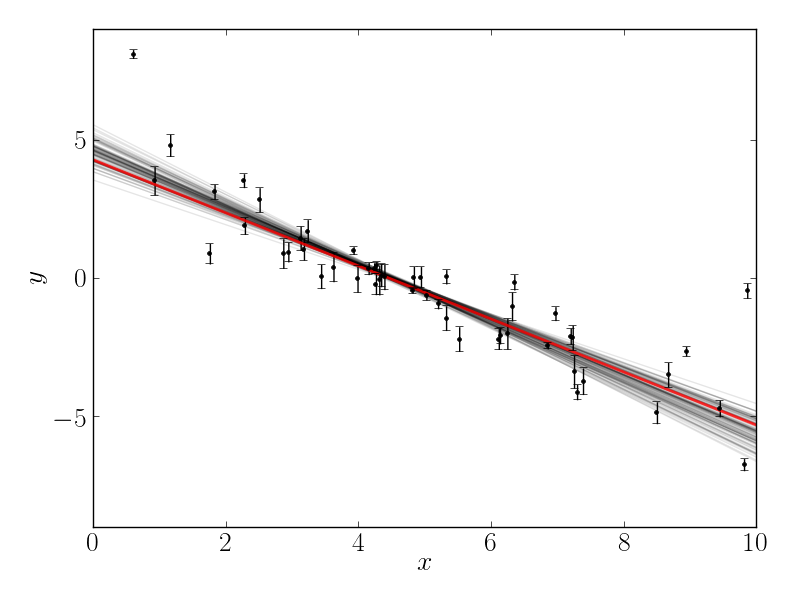
\includegraphics[width=\textwidth]{lineExample.png}
\caption{Why does this work: Fitting a line}
\label{fig:line}
\end{figure}

LA+DWH: Do we we want to put a pedagogical section in right here?

Hogg would propose a straight-line fit (possibly with intrinsic
width); showing that it can be used to de-noise noisy y-data.

\section{Assumptions and methods}

We make the following assumptions. The method we present is correct
and justifiable under these assumptions, each of which is questionable
in its own right. We return to criticize these assumptions---and the
method that flows from them---in the Discussion below.
\begin{itemize}
\item We make an assumption of \emph{stationarity}; that is, that the
  stars measured at lower signal-to-noise have analogs measured at
  higher signal-to-noise.  In detail, this assumption is wrong, of
  course (for example, distant halo stars are different than local
  disk stars), but the stationarity assumption is fairly weak; as long
  as there is support in the high signal-to-noise stars for the types
  of stars seen at low signal-to-noise, the results will not be
  strongly biased, but this assumption is deep and fundamental to this
  work.
\item We assume that we have large numbers of stars, large enough that
  an empirical-Bayes or maximum-marginalized likelihood is a safe
  approximation to full Bayesian inference. This assumption will be
  least true in the least-populated parts of the \cmd. In the extreme
  case of a stellar type with only one (statistically distinct)
  exemplar in the data set (e.g. a white dwarf), this assumption will be maximally wrong.
\item We assume that the \tgas\ parallax uncertainties dominate the
  noise in any estimates of absolute magnitude. We further assume that
  the parallax and color uncertainties are Gaussian in form with
  correctly known variances. In detail, we assume that the [INSERT
    CORRECT TERMINOLOGY FROM GAIA HERE] parallax uncertainty estimates
  are correct. Here we are making use of the fact that, for
  de-noising, under-estimation of measurement noise is conservative
  (it leads to under-deconvolution).
\item We treat the \panstarrs-based three-dimensional dust maps (\citealt{green15})
  as correct in their median dust estimates, and their
  effects on color and magnitude. As we optimize the empirical-Bayes model, we iteratively update each star's
  dust correction as its updated, inferred distance. Our assumption is that these corrections are
  good enough, and uncertainties in these are not dominant, for either
  color or absolute magnitude.
\item We assume that the \cmd\ can be represented with a mixture of
  Gaussians in a particular transformed space. This mixture we fix
  (with only heuristic analysis) at 128, 512, and 2048 Gaussians in
  different experiments.
\item We make no use of stellar models; our only assumptions about
  stellar physics are generic and implicit (for example, that the
  \cmd\ is somehow smooth and compact). Dust model dependent on stellar models?
\end{itemize}

We would like to infer the true parallax $\varpi_{\true}$ for
each star given its parallax measurement $\varpi$ and associated
uncertainty $\sigma_{\varpi}$ from \tgas.
We assume (as \gaia\ suggests) that the likelihood is Gaussian
\begin{equation}
p(\varpi \given \varpi_{\true}, I) = \mathcal{N}(\varpi \given \varpi_{\true}, \sigma^2_{\varpi}) \quad ,
\label{eq:gaialike}
\end{equation}
where $I$ is a placeholder containing our assumptions, including all
uncertainty estimates, and $\mathcal{N}(x \given \mu, \sigma^2)$ is a
Gaussian function for $x$ with mean $\mu$ and variance $\sigma^2$.
This is the probability of the data given the true parallax, but we
want to flip it around and infer the true parallax, or distance, to
the star given the measured parallax and it's uncertainty. We do this
using probability theory
\begin{equation}
p(\varpi_{\true} \given \varpi, \sigma^2_{\varpi}) = \frac{1}{Z}\,p(\varpi \given \varpi_{\true}, \sigma^2_{\varpi}) \, p(\varpi_{\true}) \quad ,
\label{eq:bayes}
\end{equation}
where $p(\varpi_{\true})$ is a prior probability density (pdf) for the
parallax to the star, and $Z$ is a normalization constant.
The strength of our inference method here lies in how we generate our prior
pdf for the parallax $p(\varpi_{\true})$.
Instead of assuming a functional form for the spatial distribution of
stars in the Milky Way (\citealt{astraatmadja16b}), or relying on stellar
models (\citealt{gaia16}), we build a noise-deconvolved estimate of the color--magnitude
diagram (\cmd) from the observed colors and absolute magnitudes of our
full set of stars.
This \cmd\ model becomes, for each star---given its observed color and
magnitude (and uncertainties on those)---a prior pdf for the distance
to that star.

That said, this is \emph{not} exactly how we do the inference here.
Here we perform the inference in a two-dimensional space that is a
transform of the \cmd....[HOGG: Syntactical marker]

To generate our \cmd\ prior we use the $J$ and $K$ band photometry from \tmass, as well as the parallax from \gaia. The data are a transformation of the dust corrected absolute magnitude, and the dust corrected colors.

\begin{equation}
10^{0.2\,M^c_{J,n} + 2} = \varpi\,10^{0.2J^c_n}
\label{eq:transform}
\end{equation}

The transformation of the dust corrected absolute magnitude, Equation \ref{eq:transform}, is required to to keep the uncertainties gaussian, which, under some assumptions along with this transformation, we maintain. Gaussian uncertainties are required to use \xd\, more about this and our dust corrections below.

Our true, latent values are the true $J-K$ color $C_n$ and the true $J$ band absolute magnitude $M_{J,n}$ for each star, which we encapsulate in the true vector $\vec{Y}$. The observed data is the dust corrected $J-K$ color $(J-K)^c_n$, the \gaia\ parallax $\varpi_n$ in units of $[mas]$, and the dust corrected $J$ band magnitude $J^c_n$, which we encapsulate in the data vector $\vec{y}$. Our prior assumptions $I$ are the uncertainties in each of these measurements, as well as the Greene dust map

\begin{equation}
\begin{aligned}
\mathrm{true \, vector} \quad &\vec{Y} = [10^{0.2\,M_{J,n} + 2}, C_n] \\
\mathrm{data \, vector} \quad &\vec{y} = [\varpi_n\,10^{0.2J^c_n}, (J- K)^c_n] \;  n \in \mathrm{stars} \\
\mathrm{with \; apparent \; magnitude} \quad &J^c_n = J_n - Q_J\,E(B-V)_n \\
\mathrm{and \; color} \quad &(J - K)^c_n = J_n - K_n - Q_{JK}\,E(B-V)_n \\
\mathrm{assumptions} \quad &I = \left\{\left\{\sigma^2_{\varpi, n}\right\}, \left\{\sigma^2_{J,n}\right\}, \left\{\sigma^2_{K,n}\right\}, \mathrm{Dust \, Map}\right\}
\end{aligned}
\label{eq:data}
\end{equation}

where $E(B-V)_n$ is the output of the Green et al dust model, and $Q_{\lambda}$ is the correction factor for a photometric band assuming some reddening law.

Working with these variables, we then have a likelihood for the data, encapsulating both the \gaia\ parallaxes and \tmass\ photometry of

\begin{equation}
p(\vec{y} \given \vec{Y}) = \mathcal{N}(\vec{y} \given \vec{Y}, \sigma_{\vec{y}})
\label{eq:fulllike}
\end{equation}

To generate our prior, we fit the data in the slightly transformed \cmd\ space, Equation \ref{eq:transform}, using \xd\ which deconvolves the data with its uncertainties, which are heterogeneous measurement uncertainties. It generates the denoised, underlying distribution from which the uncertain data were drawn from. It represents the distribution as a mixture of gaussians which maximizes the marginalized likelihood of the data, marginalized over the true data.

\xd\ generates the gaussian parameters

\begin{eqnarray}
\alpha &=& \left\{\mathrm{amp}_k, \mu_k, V_k\right\}_{k=1}^K \; k \in \mathrm{Gaussians} \nonumber\\
       &=& \argmax_{\alpha} \, \Pi_n \, p(\vec{y}_n \given \alpha) \nonumber\\
       &=& \argmax_{\alpha} \, \Pi_n \, \int p(\vec{y}_n \given \vec{Y}_n) \, p(\vec{Y} \given \alpha)\mathrm{d\vec{Y}}
\label{eq:xdmml}
\end{eqnarray}

To infer $\varpi_{\true}$ from the likelihood of the \gaia\ data, Equation \ref{eq:gaialike}, we first do the inference in the 2D space of the \cmd

\begin{equation}
p(\vec{Y} \given \vec{y}, \alpha) = \frac{1}{Z} \, p(\vec{y} \given \vec{Y}) \, p(\vec{Y} \given \alpha)
\label{eq:posterior}
\end{equation}

We then project the 2D posterior into the 1D absolute magnitude/parallax space

\begin{eqnarray}
p(\vec{Y}_0 \given \vec{y}, \alpha) &\rightarrow& p(\varpi_{\true} \given y, \alpha) \, f(\varpi_{\true}) \\
f(\varpi_{\true}) &=& \begin{cases}
              1 \quad \mathrm{if} \quad -2 < \mathrm{log}_{10} \varpi_{true} < 2\\
              0 \quad \mathrm{otherwise}
              \end{cases}
\label{eq:parallaxPost}
\end{eqnarray}

And with a jacobian this becomes a posterior on distance to the star if you wish.

Crossvalidation?

\section{Data and results}
\begin{figure}
\centering
  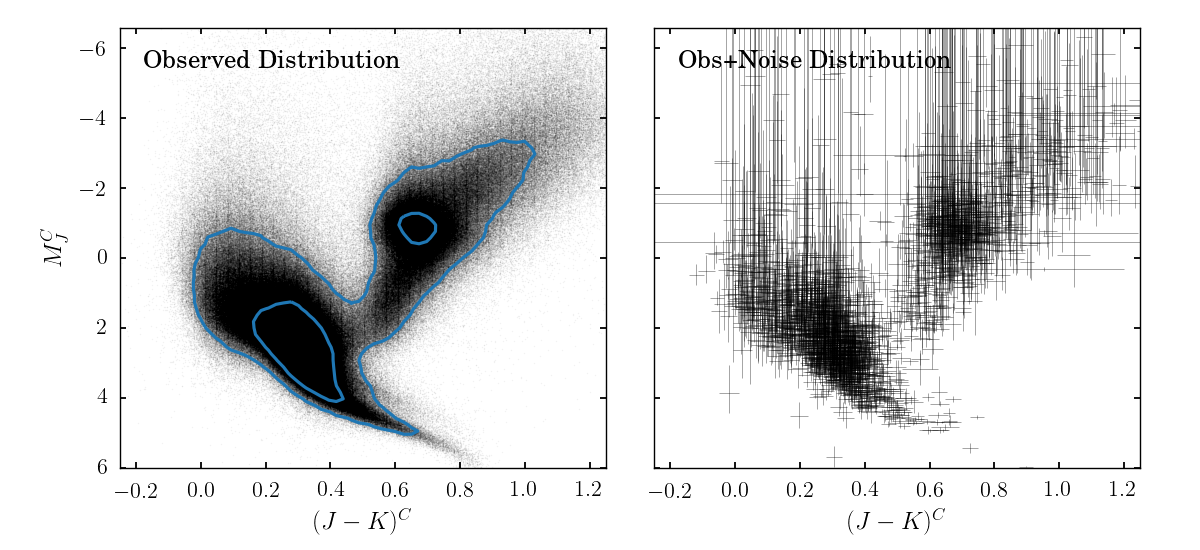
\includegraphics[width=\textwidth]{data.png}
\caption{The observed \cmd: point estimates on the left and including error bars on the right.}
\label{fig:data}
\end{figure}

We use stars crossmatched in TGAS, 2MASS and within the observing footprint of \panstarrs\ to access the Greene 3D dust model. We require the photometry have real values and nonzero, real errors, and remove a small selection of \tmass\ stars that have zero color and zero J band magnitude.

\subsection{Dust}

\begin{figure}
\centering
  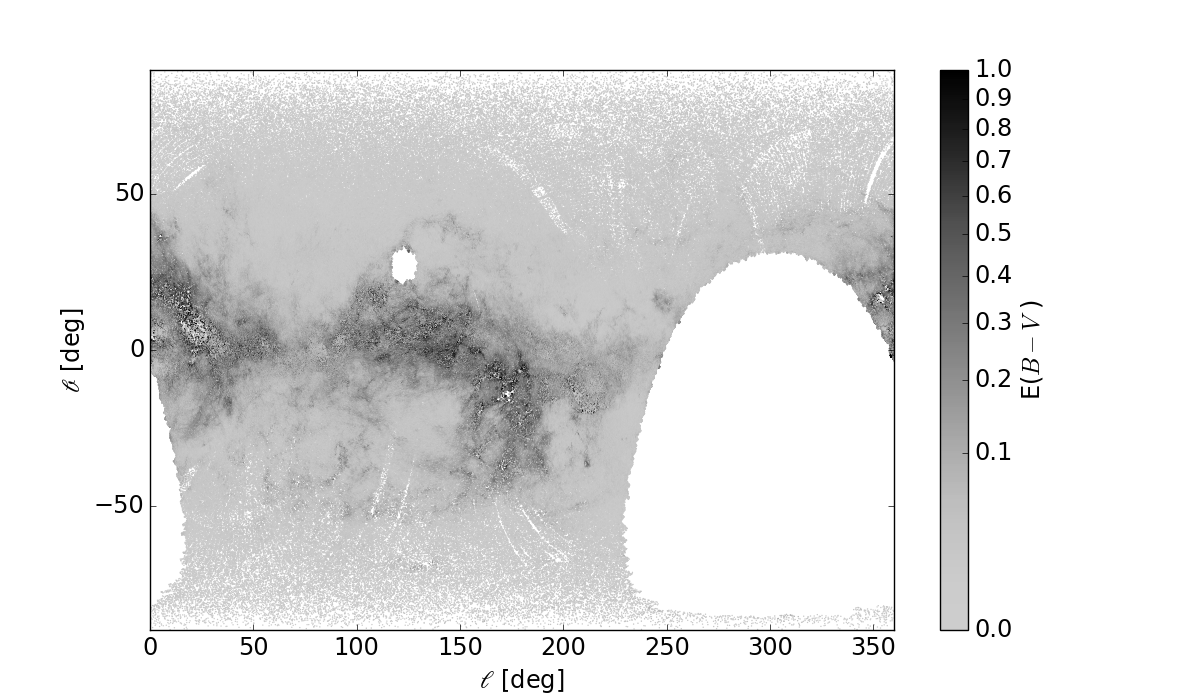
\includegraphics[width=\textwidth]{dust.png}
\caption{The converged dust values at the 5\% distance projected on the l,b galactic coordinates. This shows both the footprint of our analysis as well as the dust values we used. Each point represents a single star in our cross matched catalog. The large missing areas are due to the lack of dust values from \panstarrs\ since it only looked above -30 degrees in dec }
\label{fig:dust}
\end{figure}


We correct for dust using 3D Bayestar (Schlafly+Finkbeiner) with an estimate of the distance from iteratively sampling our posterior distances. Dust corrections are non trivial for stars with poor signal to noise. Stars with poor signal to noise have a likelihood that is consistent with infinite distance and can therefore have severe dust corrections. This is most obvious in the giant stars, which tend to have the lowest signal to noise, and can therefore have dust corrections $> 2$ magnitudes. To apply a dust correction to the \tmass\ photometry, we first generate our prior using the observed, attenuated photometry. Using this raw prior we infer more precise distances to all the stars which we can use to get a measurement of dust. This approach minimizes severe distances from the likelihoods alone and their associated severe dust corrections. With more these more precise distance posteriors, we take the $5\%$ quantile of each distance posterior, so the closest bit of the posterior, and sample the Green et al 3D dust map at that distance. For each distance we take the median of the samples of the dust model. We apply each dust correction to our \tmass\ photometry given by Equation \ref{eq:data} where $Q_{\lambda}$ = [0.709, 0.302] for bands [J, K] respectively, taken from table (REF TABLE SFD), and $E(B-V)$ is the output of the Green et al dust models. We then regenerate our prior using the dust corrected photometry. We do not update the errors, but keep them the same as before the dust correction, which is wrong and under representing our errors but this leads again to a lighter deconvolution (Do we want to change this and add in the covariance for the dust?). We iterate this process 10 times, however the dust values seem to converge after about 2-3 iterations. Should I quote some statistics about the dust corrections? mostly small? maybe difference before after correcting for distance?

\subsection{Prior}
\begin{figure}
\centering
  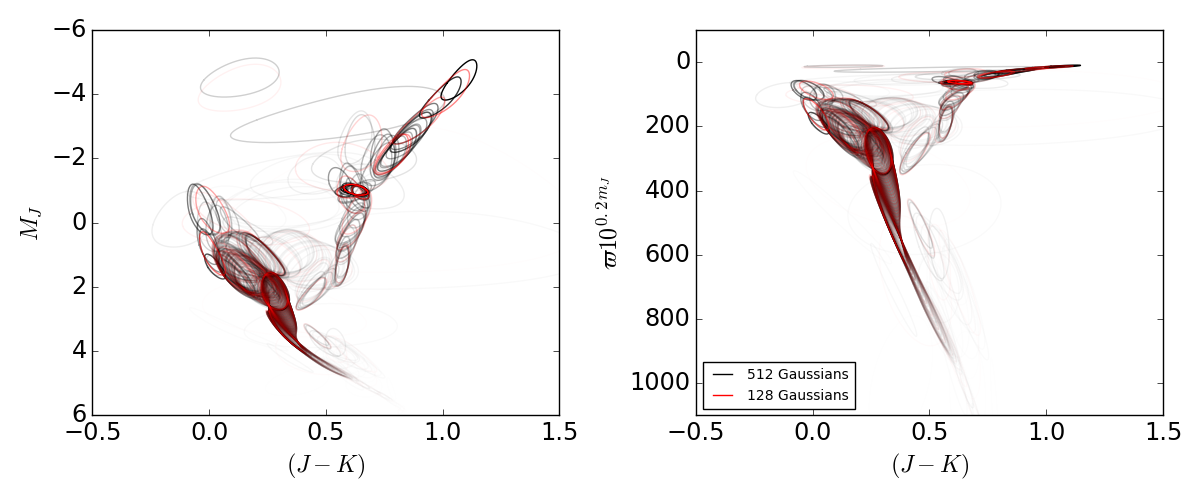
\includegraphics[width=\textwidth]{priorNgaussComparison.png}
\caption{Prior: the XD generated mixture of gaussians we use as our prior}
\label{fig:prior}
\end{figure}


LMA: what are our results?
\subsection{Distances to M67}
\begin{figure}
\centering
  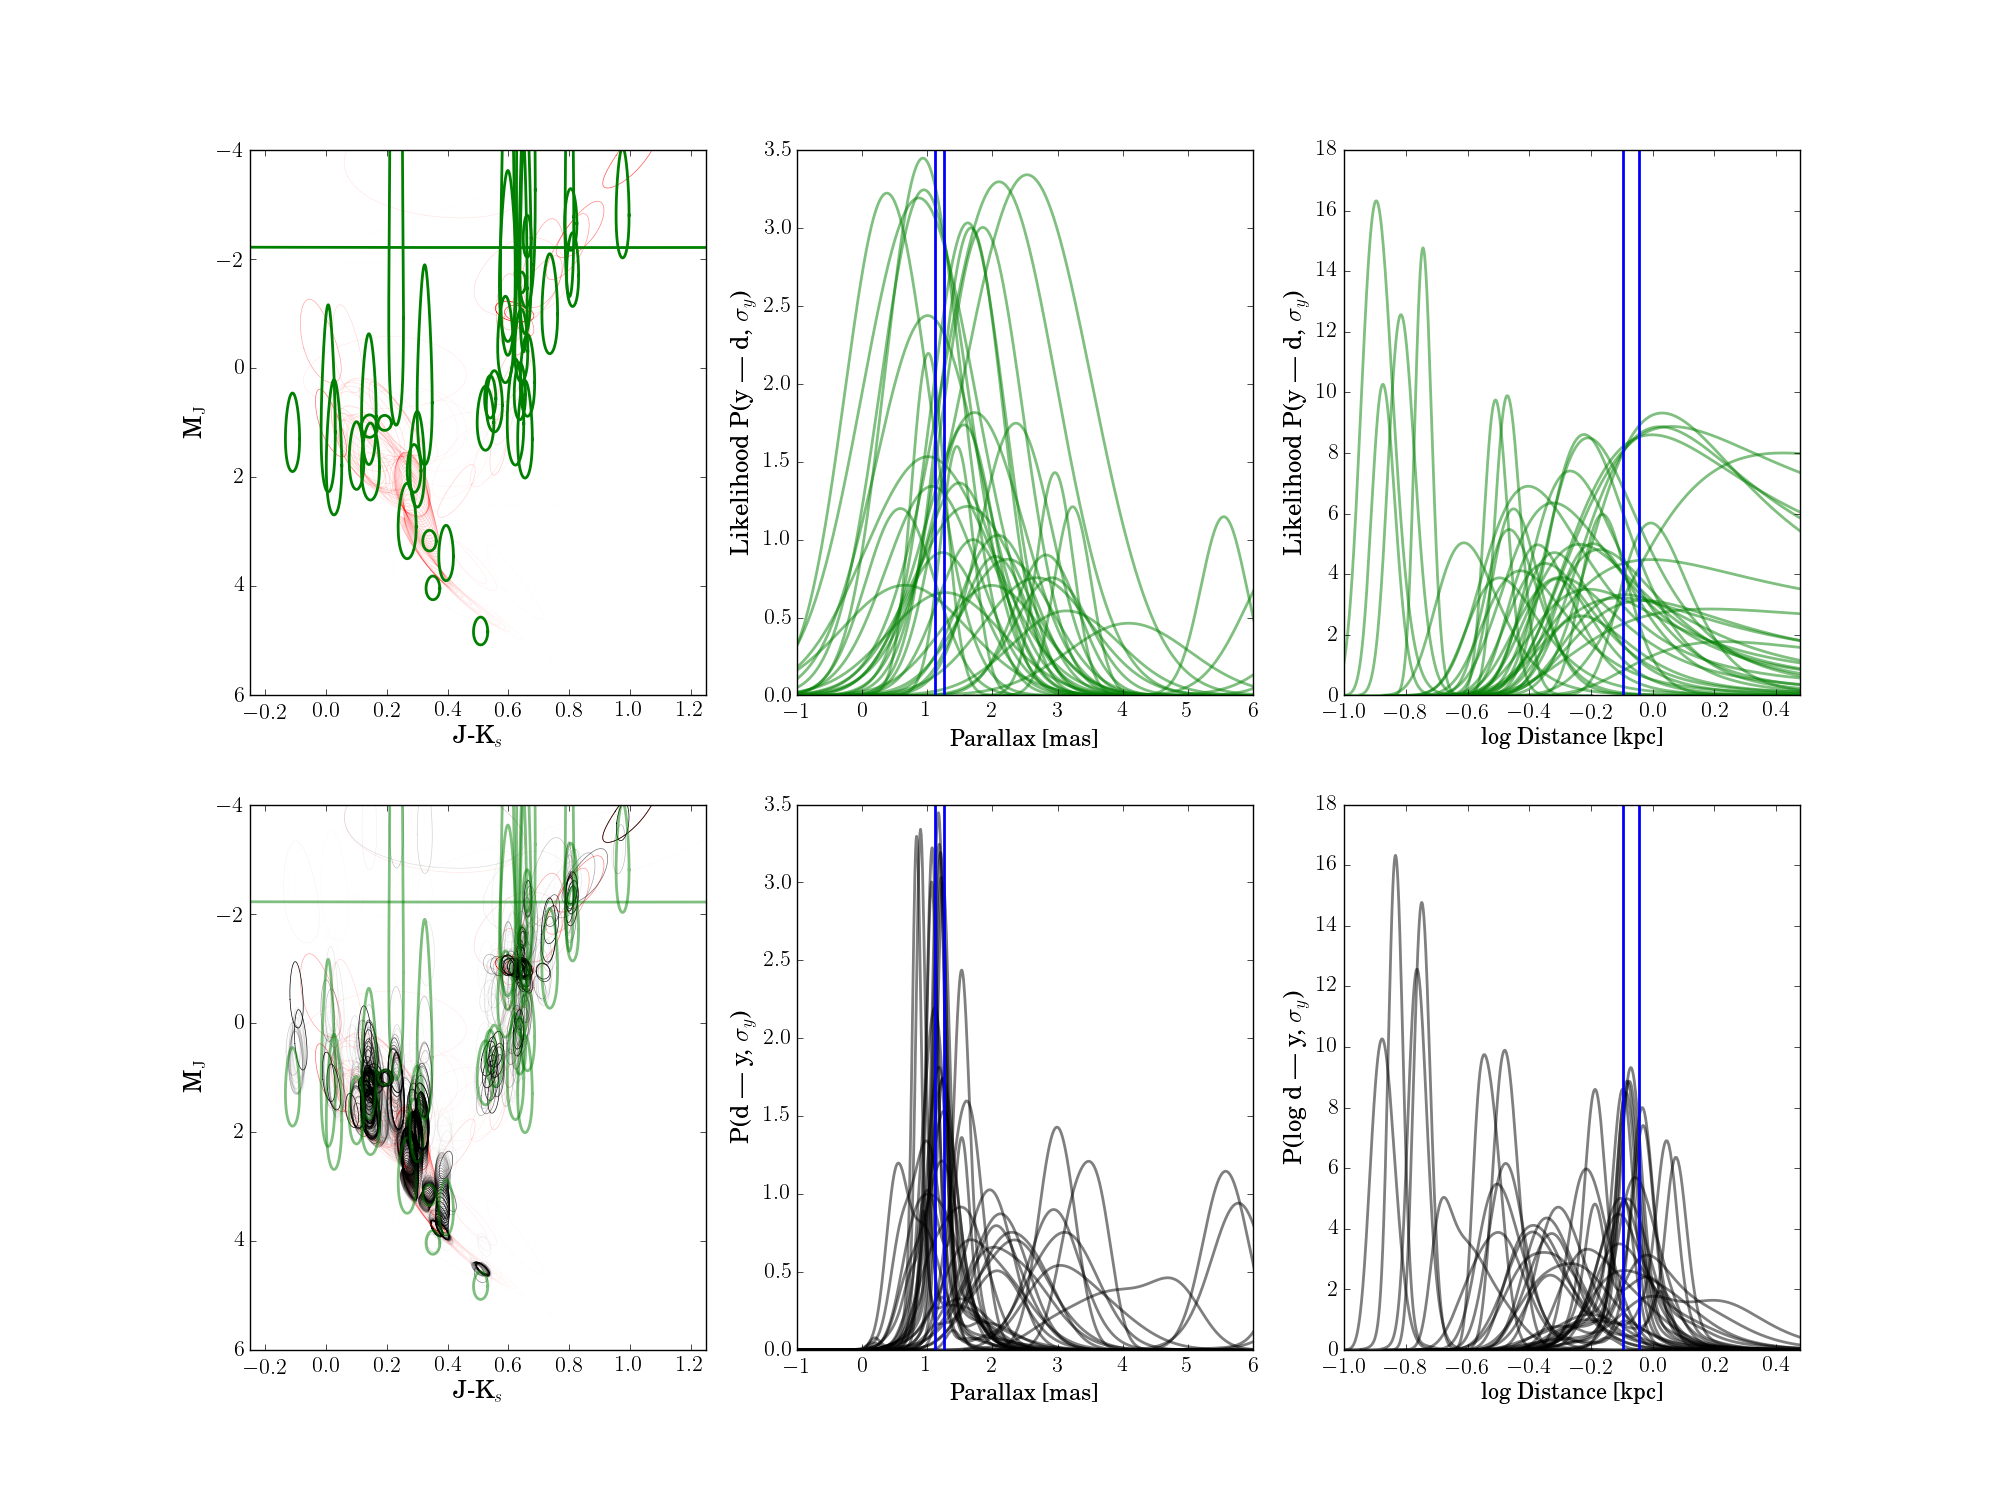
\includegraphics[width=\textwidth]{distancesM67.png}
\caption{Proof of concept: parallax inference to the open cluster M67}
\label{fig:m67}
\end{figure}

As proof of concept we inferred the distances to stars in the open cluster M67. It is an open cluster in the constellation Cancer and is estimated to be 3-5 billion years old and 800-900 pc away. Previous work has estimated that bad things happen if you try to infer a distance as the inverse of the observed (noisy) parallax when the signal to noise of the parallax measurement drops below 5. With \gaia\ parallaxes having a minimum uncertainty of about 0.3 mas, for stars with the most certain parallaxes, the SN reaches 5 at about 700 pc, right where this cluster lies. So it is a great test case for comparing parallax inferences with or without a prior. We made a window of 1 degree squared on the sky with the cluster M67 lying in the middle. The cluster is visibly obvious as a clustering of stars in a visualization of the \gaia\ data in 2D on the sky. With our converged dust values, and it's associated prior, we calculate the posterior of the true parallaxes to the stars within this window on the sky around M67. Figure XXX shows the comparison of the likelihoods and posteriors. The vertical lines bracket the parallaxes of, or distances to, the stars associated with the cluster. The likelihoods of the observed parallaxes are far broader and the cluster is not obvious at all. In the posteriors there is a sharp peak in the probability at the previously determined distance to the cluster, the vertical lines, for far more stars than the likelihoods would imply. Our prior is not only making parallaxes more precise but also (possibly) increasing the accuracy. Too strong?


\begin{figure}
\centering
  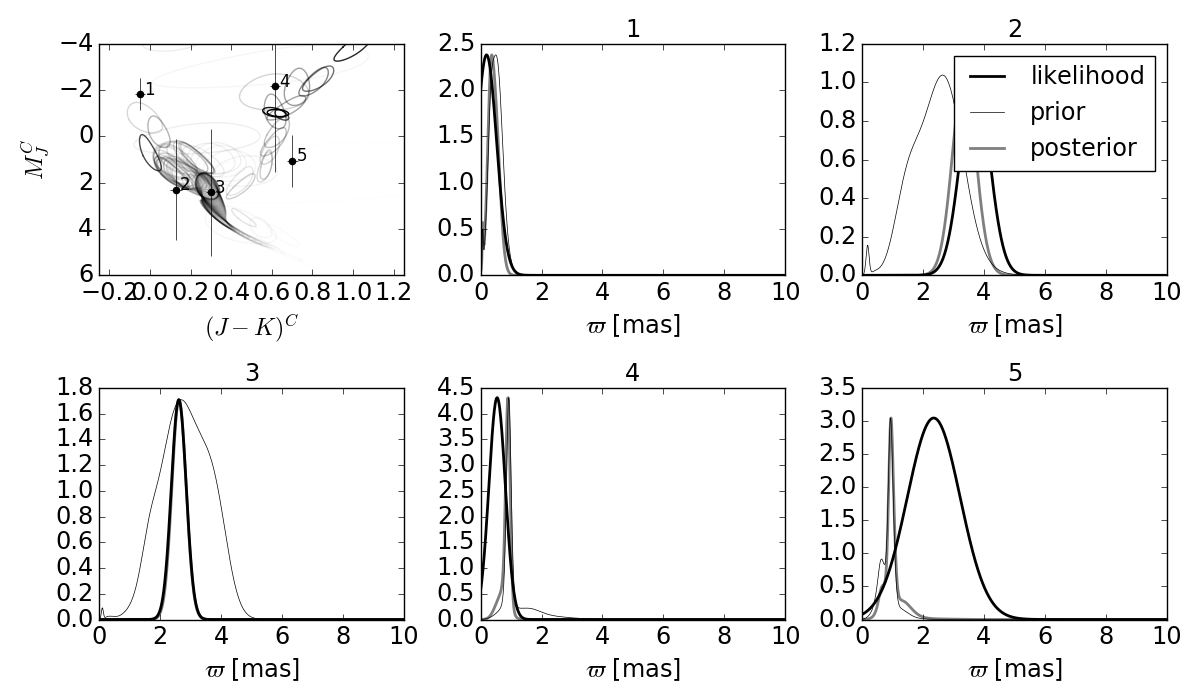
\includegraphics[width=\textwidth]{posterior.png}
\caption{5 example posteriors showing the priors and likelihoods as well}
\label{fig:posterior}
\end{figure}


\subsection{Output data}
DWH: Placeholder for the output format for our data products.


\section{Discussion}

We have shown that it is possible to obtain photometric parallaxes for
distant stars in the \gaia\ \tgas\ data without any use of physical stellar
models, nor models of the Milky Way.
That is, the geometric parallaxes can calibrate a set of photometric
models that are purely statistical---a model of the data rather than
a model of stars \foreign{per se}.
This opens up the possibility of completing the goals of the \gaia\ Mission
without building in unnecessary assumptions about the mechanical properties
of stars or the Galaxy.

We obtained the photometric parallaxes in this project
by building a data-driven model of the
color--magnitude diagram (\cmd) of the stars in the \tgas\ data set,
and using it as a prior pdf for Bayesian interences.
The posterior pdfs for distance that we obtain are, in general, much
narrower than the likelihood functions delivered by the
\gaia\ Mission, and therefore the distance estimates (or,
equivalently, parallax estimates) are much more precise.
It is not surprising that a Bayesian inference provides more
precise inferences than the likelihood function alone; Bayesian
inferences bring in new information that decrease variance (but
often introduce bias).
We have shown that, in addition to pure precision improvements, at
least some aspects of \emph{accuracy} have been improved as well, by
showing that the posterior distance estimates to stars in stellar
clusters [HOGG: Is this too general?] are much more clustered than likelihood-based distance
estimates.

Although we have not performed principled hierarchical Bayesian inference in this
project, we built our prior for each star's distance by
performing a statistically responsible deconvolution
of the \gaia\ \tgas\ data that is justifiable under a clear set of
assumptions.
This deconvolution makes use of a reasonable noise model and an
assumption of stationarity to shrink the parallax uncertainties, and
do so dramatically for the stars measured at lower signal-to-noise.
Because the method we use (Extreme Deconvolution or \xd, which is
an Empirical Bayesian maximum-marginalized-likelihood estimator) accounts for
heteroskedastic noise, we were able to build our photometric parallax
model---which is a model of the \cmd---using
all the data, not just the data with the highest signal-to-noise or
largest parallaxes.
That is, the model for the \cmd\ we have built is representative for
the \tgas\ Catalog.
Inasmuch as that is true, we expect any (sensible) distance estimates
we generate from our distance posterior pdfs to be weakly biased.

The Empirical Bayesian methodology is a good approximation to full
hierarchical inference in the limit of large numbers of data points.
That is, when no individual star is carrying a lot of weight in the
model of the \cmd.
With its millions of stars, the \tgas\ Catalog may appear to safely
live in this limit.
However, because there are parts of the \cmd\ that are poorly populated,
even in \tgas, the Empirical Bayes approximation may be bad for some
color ranges.
In particular, there appear to be essentially no white dwarf stars,
and other classes (like hot main-sequence stars) have few to no exemplars
in the data set at high signal-to-noise (in parallax).
For all these reasons, we do think that this approximation is not perfectly
safe, and it is a goal to explore full hierarchical modeling in the coming
years (and see, for example, Leistedt et al. in preparation).

In some sense, the biggest limitation of the data-driven \cmd\ model
created in this project is that we made no use of any kind of \tgas\ selection
function or completeness estimate or inverse-selection-volume corrections.
That is, the model is a model of the \tgas\ Catalog
(or really the \tgas--\tmass\ intersection), not of the stars in
the Milky Way, nor any volume-limited subsample of the Milky Way.
Importantly, because we used \emph{all} of the stars in the \tgas--\tmass\
intersection, the model \emph{is} representive of the full catalog,
even the distant parts, where all the parallaxes are measured at low
signal-to-noise.
This is in contrast to techniques that might build the model from only
the high signal-to-noise sources; such a model would be biased towards
stellar types and compositions found locally, lower-luminosity stars,
and stars which happened to get good parallaxes.
However, our use of the entire \tgas--\tmass\ intersection without
any selection function restricts the use of our \cmd\ model as a prior
to inferences within that same \tgas--\tmass\ intersection.
For example, it would be biasing to use this same prior to infer
distances for the full billion-star catalog released in \gaia\ DR1
alongside \tgas, or for stars fainter or brighter or bluer than those
included in the \tgas--\tmass\ intersection.

The outputs of this project include posterior pdfs and posterior
samplings for stellar parallaxes or distances.
It is tempting to treat these outputs as equivalent to some kind of catalog of
measurements, as we treated the original parallax measurements from \tgas.
That is, it is tempting to treat these as simply ``better'' measurements.
Taken one star at a time, this is permitted and true, and the basis for our
claim that we have de-noised the \tgas\ Catalog.
However, there are important differences, as there are with all
probabilistic catalogs (\citealt{hogg11}; \citealt{portillo17}), between the
measurements and the de-noised measurements.
The most important difference, for users of our output, between our
output and the \tgas\ data input, is that the \tgas\ data is the representation
of a likelihood function, whereas our ouptut is a
representation of a posterior pdf, one per star.
If used naively, posterior information can lead to serious statistical
errors, because each data point has had a prior multiplied in.
Effectively multiplicative uses of the data will effectively take the prior
pdf to a large power.
We have (in previous work)
given examples of correct uses of posterior samplings or pdfs
for subsequent inferences (\citealt{hogg08}; \citealt{dfm14}); we
encourage power-users to consult those methodological
contributions before engaging with these outputs.

Come back to the assumptions. What happens if we change or violate them?

Long discussion of the noise model. We took serious short-cuts. Call out to Boris.

Long discussion of dust.

Some discussion of possible failure modes. Including very rare kinds of stars.

Number of gaussians in \xd, and the w parameter. That we set them heuristically.

Talk about structures in CMD; red bump - acknowledge Ana ! s
What's That Feature? Similarly; Fraction of stars in various parts of the diagram?

Compare with literature stellar models

How this compares to other Bayesian attempts at inferring distances,
like, eg, the Tri--Coryn papers. Favorably! And with \emph{fewer}
assumptions, in fact!

\acknowledgments It is a pleasure to thank
  Ana Bonaca (Harvard),
  Andy Casey (Monash),
and the attendees at the Stars Group Meeting at the Flatiron Institute
Center for Computational Astrophysics for comments and input.
This project was developed in part at the 2016 \acronym{NYC} Gaia Sprint, hosted
by the Center for Computational Astrophysics at the Simons Foundation
in New York City.

This work has made use of data from the European Space Agency (\acronym{ESA})
mission \gaia\footnote{\url{http://www.cosmos.esa.int/gaia}}, processed by the Gaia
Data Processing and Analysis Consortium\footnote{\url{http://www.cosmos.esa.int/web/gaia/dpac/consortium}} (\acronym{DPAC}). Funding for the
\acronym{DPAC} has been provided by national institutions, in particular the
institutions participating in the Gaia Multilateral Agreement.

This publication makes use of data products from the Two Micron All
Sky Survey, which is a joint project of the
University of Massachusetts and the Infrared Processing and Analysis
Center/California Institute of Technology, funded by the National
Aeronautics and Space Administration and the National Science
Foundation.

This project was partially supported by This research was partially supported by
  the \acronym{NSF} (\acronym{AST-1517237}),
  \acronym{NASA} (grant \acronym{NNX12AI50G}),
  and the Moore-Sloan Data Science Environment at \acronym{NYU}.
It made use of the \acronym{NASA} Astrophysics Data System.
All the code used in this project is available online\footnote{\url{https://github.com/andersdot/stellarTwins}} under an open-source license.

%% \appendix
%% \section{Appendix material}

\bibliography{gaia}

\clearpage

\end{document}



%%
%% End of file `sample.tex'.
